% CS 550: Foundations of Machine Learning -- Mathematics cheat sheet
% Two landscape pages, styled after the Posit (RStudio) cheat sheets.
% Notation follows Strang (ILA) and Deisenroth, Faisal & Ong (MML).
\documentclass[9pt]{extarticle}

\usepackage[landscape,letterpaper,margin=0.35in,top=0.3in,bottom=0.3in]{geometry}
\usepackage[default]{sourcesanspro}
\usepackage[T1]{fontenc}
\usepackage{amsmath,amssymb,mathtools,bm}
\usepackage{multicol}
\usepackage{enumitem}
\usepackage{tikz}
\usepackage{pgfplots}
\pgfplotsset{compat=1.18}
\usetikzlibrary{calc,arrows.meta,angles,quotes,decorations.pathreplacing}

\pagestyle{empty}
\setlength{\parindent}{0pt}
\setlength{\parskip}{2pt}
\setlength{\columnsep}{0.22in}
\setlength{\columnseprule}{0.4pt}
\raggedcolumns
\setlist{nosep,leftmargin=1em,label=\textcolor{pblue}{\tiny$\blacksquare$}}
\setlength{\abovedisplayskip}{2pt}
\setlength{\belowdisplayskip}{2pt}
\setlength{\abovedisplayshortskip}{1pt}
\setlength{\belowdisplayshortskip}{1pt}

% ---------------------------------------------------------------- colors
\definecolor{pblue}{HTML}{447099}
\definecolor{porange}{HTML}{EE6331}
\definecolor{pgreen}{HTML}{72994E}
\definecolor{pyellow}{HTML}{E7B10A}
\definecolor{ppurple}{HTML}{9A4665}
\definecolor{plight}{HTML}{CFD9E3}
\definecolor{pdark}{HTML}{404041}
\definecolor{pgray}{HTML}{A2A2A2}
\colorlet{columnseprulecolor}{plight}

% ---------------------------------------------------------------- notation
% Vectors: bold lower case (MML); Strang writes them upright, e.g. v.
% Matrices: bold upper case (MML); Strang writes them upright, e.g. A.
\newcommand{\V}[1]{\bm{#1}}
\newcommand{\M}[1]{\bm{#1}}
\newcommand{\va}{\V{a}}  \newcommand{\vb}{\V{b}}  \newcommand{\vd}{\V{d}}
\newcommand{\ve}{\V{e}}  \newcommand{\vp}{\V{p}}  \newcommand{\vq}{\V{q}}
\newcommand{\vu}{\V{u}}  \newcommand{\vv}{\V{v}}  \newcommand{\vw}{\V{w}}
\newcommand{\vx}{\V{x}}  \newcommand{\vy}{\V{y}}  \newcommand{\vz}{\V{z}}
\newcommand{\vzero}{\V{0}}
\newcommand{\mA}{\M{A}} \newcommand{\mB}{\M{B}} \newcommand{\mC}{\M{C}}
\newcommand{\mI}{\M{I}} \newcommand{\mP}{\M{P}} \newcommand{\mQ}{\M{Q}}
\newcommand{\mR}{\M{R}} \newcommand{\mX}{\M{X}} \newcommand{\mH}{\M{H}}
\newcommand{\mLambda}{\M{\Lambda}} \newcommand{\mJ}{\M{J}}
\newcommand{\inv}{^{-1}}
\newcommand{\R}{\mathbb{R}}
\newcommand{\norm}[1]{\lVert #1 \rVert}
\newcommand{\tr}{^{\mathsf T}}
\newcommand{\abs}[1]{\lvert #1 \rvert}
\newcommand{\ip}[2]{\langle #1, #2 \rangle}
\DeclareMathOperator{\colsp}{\mathbf{C}}
\DeclareMathOperator{\nullsp}{\mathbf{N}}
\DeclareMathOperator{\spn}{span}

% ---------------------------------------------------------------- layout
\newcommand{\sheettitle}[2]{%
  \noindent\begin{tikzpicture}
    \fill[pblue] (0,0) rectangle (\linewidth,0.75);
    \node[anchor=west,text=white,font=\bfseries\Large] at (0.25,0.375) {#1};
    \node[anchor=east,text=white,font=\small] at (\linewidth-0.25,0.375) {#2};
  \end{tikzpicture}\par\vspace{2pt}}

\newcommand{\sect}[1]{%
  \par\vspace{4pt}{\color{pblue}\bfseries\large #1}\par\vspace{-2pt}%
  {\color{pblue}\rule{\linewidth}{1pt}}\par\vspace{1pt}}

\newcommand{\topic}[1]{\par\vspace{2pt}{\color{porange}\bfseries #1}\quad}

\newcommand{\note}[1]{{\color{pdark!80}\footnotesize #1}}

% ---------------------------------------------------------------- matrix pictures
% Unit = one cell. \cell{row}{col}{fill}, \zcell{row}{col} (zero entry).
\tikzset{mat/.style={x=0.24cm,y=0.24cm,baseline={(0,-1.6)}}}
\newcommand{\cell}[3]{%
  \fill[#3,rounded corners=0.5pt] ({#2-1+0.08},{-(#1)+1-0.08}) rectangle ({#2-0.08},{-(#1)+0.08});}
\newcommand{\zcell}[2]{%
  \draw[plight,line width=0.3pt,rounded corners=0.5pt] ({#2-1+0.08},{-(#1)+1-0.08}) rectangle ({#2-0.08},{-(#1)+0.08});}
\newcommand{\grid}[3]{%
  \foreach \ii in {1,...,#1}{\foreach \jj in {1,...,#2}{\cell{\ii}{\jj}{#3}}}}
\newcommand{\zgrid}[2]{%
  \foreach \ii in {1,...,#1}{\foreach \jj in {1,...,#2}{\zcell{\ii}{\jj}}}}
\newcommand{\lbl}[3]{\node[font=\scriptsize,anchor=north] at (#1,#2) {#3};}

\begin{document}
\footnotesize
%%%%%%%%%%%%%%%%%%%%%%%%%%%%%%%%%%%%%%%%%%%%%%%%%%%%%%%%%%%%%%%%%%%%%%%%%%%%%%%%
% PAGE 1
%%%%%%%%%%%%%%%%%%%%%%%%%%%%%%%%%%%%%%%%%%%%%%%%%%%%%%%%%%%%%%%%%%%%%%%%%%%%%%%%
\sheettitle{Math for ML Cheat Sheet: Linear Algebra  (v1.0)}{CS 550 \textbullet{} Foundations of Machine Learning}

\begin{multicols*}{3}

\sect{Notation}
\begin{tabular}{@{}l@{\;\;}l@{}}
  $\vx\in\R^n$ & column vector, entries $x_1,\dots,x_n$ (Strang: $\mathbf{x}$ or $x$)\\
  $\mA\in\R^{m\times n}$ & matrix, $m$ rows, $n$ columns, entry $a_{ij}$ (Strang: $A$)\\
  $\va_j$, $\va_i\tr$ & column $j$ / row $i$ of $\mA$ \\
  $\vx\tr$ & transpose: row vector \\
  $\ve_i$ & $i$-th standard basis vector; $\mI$ = identity\\
  $\vx\tr\vy = \vx\cdot\vy = \ip{\vx}{\vy}$ & dot (inner) product
\end{tabular}

\sect{Vectors}
\topic{Linear combination} of $\vv_1,\dots,\vv_k\in\R^n$ with scalars $c_1,\dots,c_k$:
\[ c_1\vv_1 + c_2\vv_2 + \dots + c_k\vv_k . \]
$\spn\{\vv_1,\dots,\vv_k\}$ = set of \emph{all} linear combinations. The vectors are
\emph{linearly independent} if $\sum_i c_i\vv_i = \vzero$ only when all $c_i=0$.

\topic{Dot product}
\[ \vx\tr\vy = \sum_{i=1}^n x_i y_i = x_1y_1+\dots+x_ny_n \in\R . \]
Symmetric, linear in each argument, $\vx\tr\vx = \norm{\vx}_2^2 \ge 0$.

\begin{minipage}[c]{0.52\linewidth}
\topic{Dot product and angle}
\[ \vx\tr\vy = \norm{\vx}_2\,\norm{\vy}_2\cos\theta \]
\[ \cos\theta = \frac{\vx\tr\vy}{\norm{\vx}_2\norm{\vy}_2} \]
$\vx\tr\vy>0$: acute, $=0$: \textbf{orthogonal} ($\vx\perp\vy$), $<0$: obtuse.
\end{minipage}\hfill
\begin{minipage}[c]{0.44\linewidth}
\centering
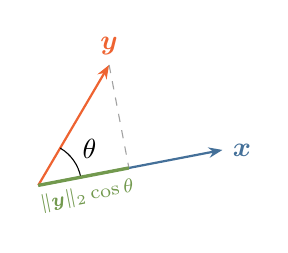
\begin{tikzpicture}[scale=0.9,>={Stealth[length=5pt]}]
  \coordinate (O) at (0,0);
  \coordinate (X) at (2.6,0.5);
  \coordinate (Y) at (1.0,1.7);
  \draw[->,thick,pblue] (O) -- (X) node[right] {$\vx$};
  \draw[->,thick,porange] (O) -- (Y) node[above] {$\vy$};
  \pic[draw,angle radius=0.55cm,"$\theta$",angle eccentricity=1.45] {angle=X--O--Y};
  % projection of y onto x
  \coordinate (P) at ($(O)!(Y)!(X)$);
  \draw[dashed,pgray] (Y) -- (P);
  \draw[pgreen,very thick] (O) -- (P);
  \node[pgreen,below,font=\scriptsize,rotate=11] at ($(O)!0.5!(P)$) {$\norm{\vy}_2\cos\theta$};
\end{tikzpicture}
\end{minipage}

\topic{Cauchy--Schwarz inequality}
\[ \abs{\vx\tr\vy} \le \norm{\vx}_2\,\norm{\vy}_2 \]
with equality iff $\vx,\vy$ are parallel. (Equivalent to $\abs{\cos\theta}\le 1$.)

\begin{minipage}[c]{0.58\linewidth}
\topic{Norm} A function $\norm{\cdot}:\R^n\to\R$ with, for all $\vx,\vy$, $\alpha$:
\begin{enumerate}[label=\textcolor{pblue}{\arabic*.},leftmargin=1.2em]
  \item $\norm{\vx}\ge 0$ and $\norm{\vx}=0 \iff \vx=\vzero$
  \item $\norm{\alpha\vx} = \abs{\alpha}\,\norm{\vx}$
  \item $\norm{\vx+\vy}\le\norm{\vx}+\norm{\vy}$ \hfill(\textbf{triangle})
\end{enumerate}
\end{minipage}\hfill
\begin{minipage}[c]{0.38\linewidth}
\centering
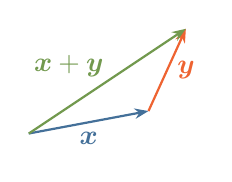
\begin{tikzpicture}[scale=0.95,>={Stealth[length=5pt]}]
  \draw[->,thick,pblue] (0,0) -- (1.6,0.3) node[midway,below] {$\vx$};
  \draw[->,thick,porange] (1.6,0.3) -- (2.1,1.4) node[midway,right] {$\vy$};
  \draw[->,thick,pgreen] (0,0) -- (2.1,1.4) node[midway,above left,inner sep=1pt] {$\vx+\vy$};
\end{tikzpicture}\\[-1pt]
\note{a side is never longer than the other two combined}
\end{minipage}

\begin{minipage}[c]{0.64\linewidth}
Common norms:\\[1pt]
$\norm{\vx}_2=\sqrt{\vx\tr\vx}=\sqrt{\textstyle\sum_i x_i^2}$ \hfill (Euclidean, default)\\
$\norm{\vx}_1=\sum_i\abs{x_i}$ \hfill (Manhattan)\\
$\norm{\vx}_\infty=\max_i\abs{x_i}$ \hfill (max)\\
\end{minipage} \hfill

\begin{minipage}[c]{0.64\linewidth}

\topic{Unit vector} $\vu = \vx/\norm{\vx}_2$ has $\norm{\vu}_2=1$.
\end{minipage}\hfill
\begin{minipage}[c]{0.32\linewidth}
\centering
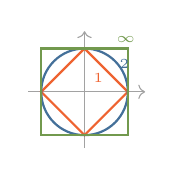
\begin{tikzpicture}[scale=0.55]
  \draw[pgray,->] (-1.3,0) -- (1.4,0); \draw[pgray,->] (0,-1.3) -- (0,1.4);
  \draw[thick,porange] (1,0) -- (0,1) -- (-1,0) -- (0,-1) -- cycle;
  \draw[thick,pblue] (0,0) circle (1);
  \draw[thick,pgreen] (-1,-1) rectangle (1,1);
  \node[font=\tiny,pgreen] at (0.95,1.2) {$\infty$};
  \node[font=\tiny,pblue] at (0.92,0.65) {$2$};
  \node[font=\tiny,porange] at (0.32,0.32) {$1$};
\end{tikzpicture}\\[-1pt]
\note{unit balls $\norm{\vx}\le 1$}
\end{minipage}

\columnbreak
%------------------------------------------------------------------------------
\sect{Matrix Multiplication}
$\mA\in\R^{m\times n}$, $\mB\in\R^{n\times p}$ $\Rightarrow$ $\mC=\mA\mB\in\R^{m\times p}$.
Inner dimensions must agree. In general $\mA\mB\ne\mB\mA$; but $(\mA\mB)\mC=\mA(\mB\mC)$.

\topic{As inner products} (row $\cdot$ column)
\[ c_{ij} = \va_i\tr\vb_j = \sum_{k=1}^n a_{ik}b_{kj} \]
\centering
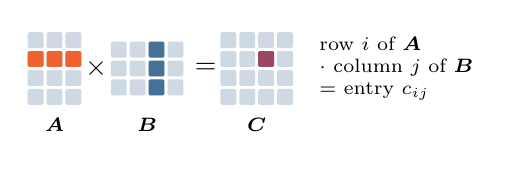
\begin{tikzpicture}[mat]
  \grid{4}{3}{plight} \foreach \j in {1,2,3}{\cell{2}{\j}{porange}}
  \lbl{1.5}{-4.1}{$\mA$}
  \node at (3.7,-2) {$\times$};
  \begin{scope}[shift={(4.4,-0.5)}]
    \grid{3}{4}{plight} \foreach \i in {1,2,3}{\cell{\i}{3}{pblue}}
    \lbl{2}{-3.6}{$\mB$}
  \end{scope}
  \node at (9.5,-2) {$=$};
  \begin{scope}[shift={(10.2,0)}]
    \grid{4}{4}{plight} \cell{2}{3}{ppurple}
    \lbl{2}{-4.1}{$\mC$}
  \end{scope}
  \node[font=\scriptsize,anchor=west,align=left] at (15,-2)
    {row $i$ of $\mA$ \\ $\cdot$ column $j$ of $\mB$\\ $=$ entry $c_{ij}$};
\end{tikzpicture}

\raggedright
\topic{As outer products} (column $\times$ row, sum of rank-one matrices)
\[ \mA\mB = \sum_{k=1}^n \va_k\,\vb_k\tr \qquad(\va_k=\text{col } k \text{ of } \mA,\ \vb_k\tr=\text{row } k \text{ of } \mB)\]
\centering
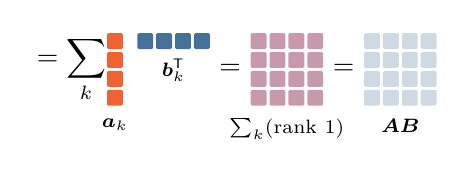
\begin{tikzpicture}[mat]
  \node at (-1.8,-2) {$=\displaystyle\sum_{k}$};
  \foreach \i in {1,...,4}{\cell{\i}{1}{porange}}
  \lbl{0.5}{-4.1}{$\va_k$}
  \begin{scope}[shift={(1.6,0)}]
    \foreach \j in {1,...,4}{\cell{1}{\j}{pblue}}
    \lbl{2}{-0.9}{$\vb_k\tr$}
  \end{scope}
  \node at (6.6,-2) {$=$};
  \begin{scope}[shift={(7.6,0)}]
    \grid{4}{4}{ppurple!55}
    \lbl{2}{-4.1}{$\sum_k(\text{rank }1)$}
  \end{scope}
  \node at (12.6,-2) {$=$};
  \begin{scope}[shift={(13.6,0)}]
    \grid{4}{4}{plight}
    \lbl{2}{-4.1}{$\mA\mB$}
  \end{scope}
\end{tikzpicture}

\raggedright
\topic{Matrix--vector: combination of columns} (Strang's view)
\[ \mA\vx = x_1\va_1 + x_2\va_2 + \dots + x_n\va_n \]
\centering
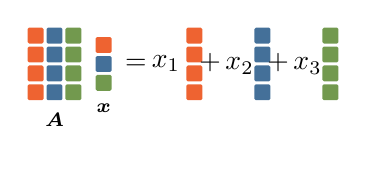
\begin{tikzpicture}[mat]
  \foreach \i in {1,...,4}{\cell{\i}{1}{porange}\cell{\i}{2}{pblue}\cell{\i}{3}{pgreen}}
  \lbl{1.5}{-4.1}{$\mA$}
  \begin{scope}[shift={(3.6,-0.5)}]
    \cell{1}{1}{porange}\cell{2}{1}{pblue}\cell{3}{1}{pgreen}
    \lbl{0.5}{-3.1}{$\vx$}
  \end{scope}
  \node at (5.8,-2) {$=$};
  \node at (7.4,-2) {$x_1$};
  \begin{scope}[shift={(8.4,0)}] \foreach \i in {1,...,4}{\cell{\i}{1}{porange}} \end{scope}
  \node at (10.6,-2) {$+\,x_2$};
  \begin{scope}[shift={(12.0,0)}] \foreach \i in {1,...,4}{\cell{\i}{1}{pblue}} \end{scope}
  \node at (14.2,-2) {$+\,x_3$};
  \begin{scope}[shift={(15.6,0)}] \foreach \i in {1,...,4}{\cell{\i}{1}{pgreen}} \end{scope}
\end{tikzpicture}

\raggedright
\sect{Transpose}
\begin{minipage}[c]{0.58\linewidth}
$(\mA\tr)_{ij}=a_{ji}$: rows become columns.
\begin{itemize}
  \item $(\mA\tr)\tr=\mA$, \ $(\mA+\mB)\tr=\mA\tr+\mB\tr$
  \item $(\mA\mB)\tr=\mB\tr\mA\tr$ \ (order reverses)
  \item $\vx\tr\vy$ is a scalar; $\vx\vy\tr$ is a matrix
  \item $(\mA\vx)\tr\vy = \vx\tr(\mA\tr\vy)$
\end{itemize}
\end{minipage}\hfill
\begin{minipage}[c]{0.38\linewidth}
\centering
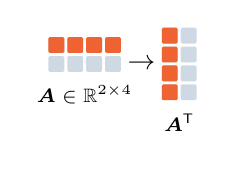
\begin{tikzpicture}[mat]
  \grid{2}{4}{plight} \foreach \j in {1,...,4}{\cell{1}{\j}{porange}}
  \lbl{2}{-2.1}{$\mA\in\R^{2\times4}$}
  \node at (5,-1.5) {$\to$};
  \begin{scope}[shift={(6,0.5)}]
    \grid{4}{2}{plight} \foreach \i in {1,...,4}{\cell{\i}{1}{porange}}
    \lbl{1}{-4.1}{$\mA\tr$}
  \end{scope}
\end{tikzpicture}
\end{minipage}

\sect{Special Matrices}
\begin{minipage}[c]{0.66\linewidth}
\topic{Symmetric} $\mA=\mA\tr$, i.e.\ $a_{ij}=a_{ji}$ (square).
$\mA\tr\mA$ and $\mA\mA\tr$ are always symmetric. Symmetric matrices have real eigenvalues
and orthogonal eigenvectors (see p.\,2).
\end{minipage}\hfill
\begin{minipage}[c]{0.3\linewidth}
\centering

\begin{tikzpicture}[mat]
  \foreach \i in {1,2,3}{\cell{\i}{\i}{pgray}}
  \cell{1}{2}{porange}\cell{2}{1}{porange}
  \cell{1}{3}{pblue}\cell{3}{1}{pblue}
  \cell{2}{3}{pgreen}\cell{3}{2}{pgreen}
\end{tikzpicture}
\end{minipage}

\topic{Inverse} $\mA\in\R^{n\times n}$ is invertible if there is $\mA\inv$ with
$\mA\inv\mA = \mA\mA\inv = \mI$. Then $\mA\vx=\vb$ has the unique solution $\vx=\mA\inv\vb$.
\begin{itemize}
  \item invertible $\iff$ $\det\mA\ne0$ $\iff$ columns independent $\iff$ $\mA\vx=\vzero$ only for $\vx=\vzero$
  \item $(\mA\mB)\inv=\mB\inv\mA\inv$, \quad $(\mA\tr)\inv=(\mA\inv)\tr$
  \item $\begin{bmatrix} a & b\\ c& d\end{bmatrix}^{-1} = \dfrac{1}{ad-bc}\begin{bmatrix} d & -b\\ -c& a\end{bmatrix}$
\end{itemize}

\columnbreak
%------------------------------------------------------------------------------
\sect{Orthogonal Matrices}
\begin{minipage}[c]{0.6\linewidth}
\topic{Orthogonal matrix} Square $\mQ$ with \emph{orthonormal} columns
($\vq_i\tr\vq_j=0$ for $i\neq j$, $\norm{\vq_i}_2=1$):
\[ \mQ\tr\mQ = \mQ\mQ\tr = \mI, \qquad \mQ\inv=\mQ\tr. \]
\end{minipage}\hfill
\begin{minipage}[c]{0.38\linewidth}
\centering
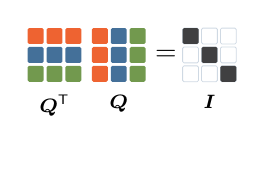
\begin{tikzpicture}[mat]
  \foreach \j in {1,2,3}{\cell{1}{\j}{porange}\cell{2}{\j}{pblue}\cell{3}{\j}{pgreen}}
  \lbl{1.5}{-3.1}{$\mQ\tr$}
  \begin{scope}[shift={(3.4,0)}]
    \foreach \i in {1,2,3}{\cell{\i}{1}{porange}\cell{\i}{2}{pblue}\cell{\i}{3}{pgreen}}
    \lbl{1.5}{-3.1}{$\mQ$}
  \end{scope}
  \node at (7.4,-1.5) {$=$};
  \begin{scope}[shift={(8.2,0)}]
    \zgrid{3}{3} \foreach \i in {1,2,3}{\cell{\i}{\i}{pdark}}
    \lbl{1.5}{-3.1}{$\mI$}
  \end{scope}
\end{tikzpicture}
\end{minipage}
Preserves lengths and angles: $\norm{\mQ\vx}_2=\norm{\vx}_2$, $(\mQ\vx)\tr(\mQ\vy)=\vx\tr\vy$.
Examples: rotations, reflections, permutations.

\begin{minipage}[c]{0.6\linewidth}
\topic{Rotation in 2D} by angle $\theta$ (counterclockwise):
\[ \mR_{\theta}=\begin{bmatrix}\cos\theta & -\sin\theta\\ \sin\theta & \cos\theta\end{bmatrix} \]
Columns = images of $\ve_1,\ve_2$.
$\mR_{\theta}\inv=\mR_{\theta}\tr=\mR_{-\theta}$, $\det\mR=1$, $\mR_{\alpha}\mR_{\beta}=\mR_{\alpha+\beta}$.
\end{minipage}\hfill
\begin{minipage}[c]{0.38\linewidth}
\centering
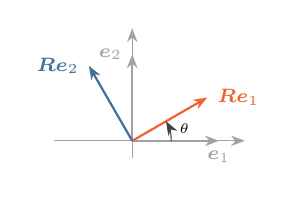
\begin{tikzpicture}[scale=1.1,>={Stealth[length=5pt]}]
  \draw[pgray,->] (-0.9,0) -- (1.3,0); \draw[pgray,->] (0,-0.2) -- (0,1.3);
  \draw[->,thick,pgray] (0,0) -- (1,0) node[below,font=\scriptsize] {$\ve_1$};
  \draw[->,thick,pgray] (0,0) -- (0,1) node[left,font=\scriptsize] {$\ve_2$};
  \draw[->,thick,porange] (0,0) -- ({cos(30)},{sin(30)}) node[right,font=\scriptsize] {$\mR\ve_1$};
  \draw[->,thick,pblue] (0,0) -- ({-sin(30)},{cos(30)}) node[left,font=\scriptsize] {$\mR\ve_2$};
  \draw[->,pdark] (0.45,0) arc (0:30:0.45); \node[font=\tiny] at (0.6,0.14) {$\theta$};
\end{tikzpicture}
\end{minipage}

\sect{Subspaces}
\topic{Vector subspace} $S\subseteq\R^n$ is a subspace if $\vzero\in S$ and it is closed under linear combinations:
\[ \vx,\vy\in S,\ \alpha,\beta\in\R \ \Rightarrow\ \alpha\vx+\beta\vy\in S . \]
Examples: lines/planes through the origin, $\spn\{\vv_1,\dots,\vv_k\}$,
column space $\colsp(\mA)=\{\mA\vx\mid\vx\in\R^n\}$, nullspace $\nullsp(\mA)=\{\vx\mid \mA\vx=\vzero,\vx\in\R^n\}$.
A \emph{basis} is an independent spanning set; its size is the \emph{dimension}.
$\vx\perp S$ means $\vx\tr\vy=0$ for all $\vy\in S$.

\sect{Orthogonal Projection}
\begin{minipage}[c]{0.5\linewidth}
\topic{Project $\vb$ onto the line through $\va$}
\[ \vp = \frac{\va\va\tr}{\va\tr\va}\,\vb = \mP\vb, \qquad \mP=\frac{\va\va\tr}{\va\tr\va}. \]
Error $\ve=\vb-\vp$ is \textbf{orthogonal} to the line: $\va\tr\ve=0$
and $\| \vb - \vp \|_2^2  = \min_{x} \| \vb - \va x\|_2^2$.
\end{minipage}\hfill
\begin{minipage}[c]{0.48\linewidth}
\centering
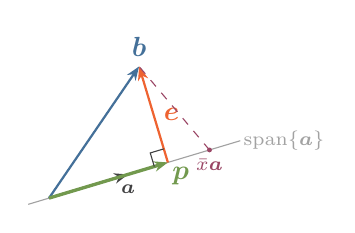
\begin{tikzpicture}[scale=0.88,>={Stealth[length=5pt]}]
  \coordinate (O) at (0,0);
  \coordinate (A) at (3.0,0.9);
  \coordinate (B) at (1.3,1.9);
  \coordinate (P) at ($(O)!(B)!(A)$);
  \coordinate (Q) at ($(O)!1.35!(P)$);
  \draw[pgray,thin] ($(O)!-0.1!(A)$) -- ($(O)!0.92!(A)$) node[right,font=\scriptsize,inner sep=1pt] {$\spn\{\va\}$};
  \draw[->,thick,pdark] (O) -- ($(O)!0.38!(A)$) node[below,font=\scriptsize] {$\va$};
  \draw[->,thick,pblue] (O) -- (B) node[above] {$\vb$};
  \draw[->,very thick,pgreen] (O) -- (P) node[below right,inner sep=1pt] {$\vp$};
  \draw[->,thick,porange] (P) -- (B) node[midway,right] {$\ve$};
  \draw[dashed,ppurple] (Q) -- (B);
  \fill[ppurple] (Q) circle (1pt);
  \node[ppurple,font=\scriptsize,below] at (Q) {$\bar x\va$};
  \pic[draw,pdark,angle radius=0.18cm] {right angle=B--P--O};
\end{tikzpicture}\\
\note{dashed: $\norm{\vb- \bar x \va}_2>\norm{\ve}_2$}
\end{minipage}

\topic{Onto a subspace $\colsp(\mA)$}
\[ \vp = \mP \vb, \quad \ve = (\mI - \mP) \vb, \quad \mP=\mA(\mA\tr\mA)\inv\mA\tr  \]
$\vp=\mA\hat\vx$ minimizes the error:
\[
  \begin{aligned}
    \hat\vx&=\arg\min_{\vx}\norm{\vb-\mA\vx}_2^2 = \arg\min_{\vx} \left(  \vx\tr\mA\tr\mA\vx - 2\vb\tr\mA\vx \right) \\
    &= (\mA\tr\mA)\inv\mA\tr\vb  
  \end{aligned}
  \]
Error $\perp$ every column: $\mA\tr\ve=\vzero$.

Orthonormal columns ($\mA=\mQ$): $\mP=\mQ\mQ\tr$, $\vp=\sum_i(\vq_i\tr\vb)\vq_i$.

\topic{Important properties}
\begin{itemize}
\item $(\mA\tr \mA)^{-1}$ exists iff columns of $\mA$ are independent
\end{itemize}


\topic{Properties of a projection matrix $\mP$}
\begin{itemize}
  \item $\mP^2=\mP$ (idempotent: projecting twice changes nothing)
  \item $\mP\tr=\mP$ (symmetric); eigenvalues are $0$ or $1$
  \item $\mI-\mP$ projects onto the orthogonal complement; $\ve=(\mI-\mP)\vb$
  \item Pythagoras: $\norm{\vb}_2^2=\norm{\vp}_2^2+\norm{\ve}_2^2$, so $\norm{\mP\vb}_2\le\norm{\vb}_2$
  \item $\vp$ is the unique closest point of the subspace to $\vb$
\end{itemize}

\end{multicols*}

%%%%%%%%%%%%%%%%%%%%%%%%%%%%%%%%%%%%%%%%%%%%%%%%%%%%%%%%%%%%%%%%%%%%%%%%%%%%%%%%
% PAGE 2
%%%%%%%%%%%%%%%%%%%%%%%%%%%%%%%%%%%%%%%%%%%%%%%%%%%%%%%%%%%%%%%%%%%%%%%%%%%%%%%%
\newpage
\sheettitle{Math for ML Cheat Sheet: Eigenvalues, Calculus \& Optimization}{References: Strang ILA \textbullet{} Deisenroth et al.\ MML}

\begin{multicols*}{3}

\sect{Eigenvalues \& Eigenvectors}
For square $\mA\in\R^{n\times n}$, a nonzero $\vx$ is an \textbf{eigenvector} with
\textbf{eigenvalue} $\lambda$ if
\[ \mA\vx=\lambda\vx \qquad(\vx\neq\vzero). \]
$\mA$ only stretches $\vx$ by $\lambda$, never changes its direction (up to sign).
\begin{itemize}
  \item eigenvalues solve $\det(\mA-\lambda\mI)=0$
  \item $\sum_i\lambda_i=\operatorname{tr}\mA$, \ $\prod_i\lambda_i=\det\mA$
  \item $\mA^k\vx=\lambda^k\vx$; \ $\mA\inv\vx=\lambda\inv\vx$
\end{itemize}

\topic{Diagonalization} If $\mA$ has $n$ \emph{independent} eigenvectors
(columns of $\mX$), eigenvalues on the diagonal of $\mLambda$:
\[ \mA = \mX\mLambda\mX\inv,\qquad \mA^k = \mX\mLambda^k\mX\inv . \]
\centering
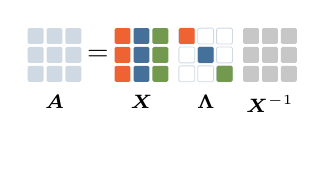
\begin{tikzpicture}[mat]
  \grid{3}{3}{plight} \lbl{1.5}{-3.1}{$\mA$}
  \node at (3.8,-1.5) {$=$};
  \begin{scope}[shift={(4.6,0)}]
    \foreach \i in {1,2,3}{\cell{\i}{1}{porange}\cell{\i}{2}{pblue}\cell{\i}{3}{pgreen}}
    \lbl{1.5}{-3.1}{$\mX$}
  \end{scope}
  \begin{scope}[shift={(8,0)}]
    \zgrid{3}{3} \cell{1}{1}{porange}\cell{2}{2}{pblue}\cell{3}{3}{pgreen}
    \lbl{1.5}{-3.1}{$\mLambda$}
  \end{scope}
  \begin{scope}[shift={(11.4,0)}]
    \grid{3}{3}{pgray!60}
    \lbl{1.5}{-3.1}{$\mX\inv$}
  \end{scope}
\end{tikzpicture}

\raggedright
\textcolor{porange}{\bfseries Not always possible!} E.g.\
$\begin{bsmallmatrix}0&1\\0&0\end{bsmallmatrix}$ has $\lambda=0$ twice but only one
eigenvector direction. Guaranteed when the $n$ eigenvalues are distinct and real, or $\mA$ is symmetric.
Eigenvalues may be complex (e.g.\ rotations).

\topic{Symmetric matrices} (spectral theorem) If $\mA=\mA\tr$: all $\lambda_i$ real,
eigenvectors can be chosen orthonormal, so $\mX=\mQ$ is orthogonal:
\[ \mA=\mQ\mLambda\mQ\tr=\sum_{i=1}^n\lambda_i\,\vq_i\vq_i\tr . \]
\centering
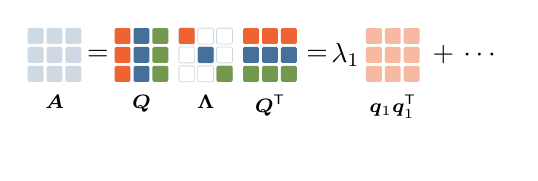
\begin{tikzpicture}[mat]
  \grid{3}{3}{plight} \lbl{1.5}{-3.1}{$\mA$}
  \node at (3.8,-1.5) {$=$};
  \begin{scope}[shift={(4.6,0)}]
    \foreach \i in {1,2,3}{\cell{\i}{1}{porange}\cell{\i}{2}{pblue}\cell{\i}{3}{pgreen}}
    \lbl{1.5}{-3.1}{$\mQ$}
  \end{scope}
  \begin{scope}[shift={(8,0)}]
    \zgrid{3}{3} \cell{1}{1}{porange}\cell{2}{2}{pblue}\cell{3}{3}{pgreen}
    \lbl{1.5}{-3.1}{$\mLambda$}
  \end{scope}
  \begin{scope}[shift={(11.4,0)}]
    \foreach \j in {1,2,3}{\cell{1}{\j}{porange}\cell{2}{\j}{pblue}\cell{3}{\j}{pgreen}}
    \lbl{1.5}{-3.1}{$\mQ\tr$}
  \end{scope}
  \node at (15.4,-1.5) {$=$};
  \node at (16.9,-1.5) {$\lambda_1$};
  \begin{scope}[shift={(17.9,0)}] \grid{3}{3}{porange!45} \lbl{1.5}{-3.1}{$\vq_1\vq_1\tr$} \end{scope}
  \node at (23.3,-1.5) {$+\,\cdots$};
\end{tikzpicture}

\raggedright
\sect{Definiteness \& Quadratic Forms}
\topic{Quadratic form} For symmetric $\mA\in\R^{n\times n}$:
\[ \vx\tr\mA\vx=\sum_{i=1}^n\sum_{j=1}^n a_{ij}x_ix_j \]
\[ \begin{bmatrix}x_1\\x_2\end{bmatrix}^{\!\top}\!\begin{bmatrix}a&b\\b&c\end{bmatrix}\!\begin{bmatrix}x_1\\x_2\end{bmatrix}
  = a x_1^2+2b\,x_1x_2+c\,x_2^2 . \]
Non-symmetric $\mA$: same form as $\tfrac12(\mA+\mA\tr)$. With $\mA=\mQ\mLambda\mQ\tr$ it is a
\textbf{sum of squares} along the eigenvectors:
\[ \vx\tr\mA\vx=\sum_{i=1}^n\lambda_i\,(\vq_i\tr\vx)^2 . \]

\topic{Positive (semi-)definite} Symmetric $\mA$ is
\begin{itemize}
  \item \textbf{PD} ($\mA\succ0$): $\vx\tr\mA\vx>0$ for all $\vx\ne\vzero$ $\iff$ all $\lambda_i>0$
  \item \textbf{PSD} ($\mA\succeq0$): $\vx\tr\mA\vx\ge0$ for all $\vx$ $\iff$ all $\lambda_i\ge0$
\end{itemize}
$\mA\tr\mA$ is always PSD (PD if the columns of $\mA$ are independent), since
$\vx\tr\mA\tr\mA\vx=\norm{\mA\vx}_2^2$. PD $\Rightarrow$ invertible.

\columnbreak
%------------------------------------------------------------------------------
\topic{Picture of a quadratic} $f(\vx)=\vx\tr\mA\vx$ with
$\mA=\begin{bsmallmatrix}0.7&-0.3\\-0.3&0.7\end{bsmallmatrix}$,
$\lambda_1=0.4$, $\vq_1=\tfrac1{\sqrt2}\begin{bsmallmatrix}1\\1\end{bsmallmatrix}$,
$\lambda_2=1$, $\vq_2=\tfrac1{\sqrt2}\begin{bsmallmatrix}1\\-1\end{bsmallmatrix}$
\note{(cf.\ \texttt{code/julia/10-quadratic.jl})}

\centering
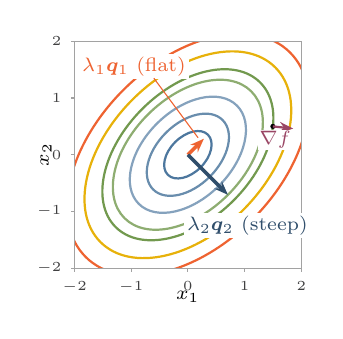
\begin{tikzpicture}[scale=0.72,>={Stealth[length=5pt]}]
  \begin{scope}
    \clip (-2,-2) rectangle (2,2);
    \foreach \c/\col in {0.1/pblue!95,0.3/pblue!80,0.6/pblue!65,1.0/pgreen!80,1.3/pgreen,1.9/pyellow,2.6/porange}{
      \draw[\col,thick,rotate=45] (0,0) ellipse ({sqrt(\c/0.4)} and {sqrt(\c)});
    }
  \end{scope}
  \draw[pgray] (-2,-2) rectangle (2,2);
  \foreach \t in {-2,-1,0,1,2}{
    \draw[pgray] (\t,-2) -- (\t,-2.06) node[below,font=\tiny,pdark] {$\t$};
    \draw[pgray] (-2,\t) -- (-2.06,\t) node[left,font=\tiny,pdark] {$\t$};}
  \node[font=\scriptsize] at (0,-2.5) {$x_1$};
  \node[font=\scriptsize,rotate=90] at (-2.5,0) {$x_2$};
  \draw[->,line width=1.3pt,porange] (0,0) -- ({0.4/sqrt(2)},{0.4/sqrt(2)});
  \draw[->,line width=1.3pt,pblue!70!black] (0,0) -- ({1/sqrt(2)},{-1/sqrt(2)});
  \node[font=\scriptsize,porange,fill=white,inner sep=1pt] at (-0.95,1.55) {$\lambda_1\vq_1$ (flat)};
  \draw[porange,thin] (-0.6,1.35) -- (0.18,0.3);
  \node[font=\scriptsize,pblue!70!black,fill=white,inner sep=1pt] at (1.05,-1.25) {$\lambda_2\vq_2$ (steep)};
  % gradient at x0 = (1.5,0.5), f = 1.3, grad = 2Ax0 = (1.8,-0.2)
  \fill (1.5,0.5) circle (1.3pt);
  \draw[->,thick,ppurple] (1.5,0.5) -- (1.86,0.46) node[below left,font=\scriptsize,fill=white,inner sep=0.5pt] {$\nabla f$};
\end{tikzpicture}\hspace{2pt}%
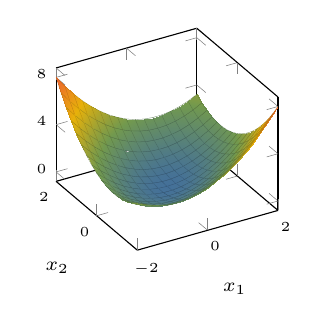
\begin{tikzpicture}
  \begin{axis}[width=4.4cm,height=4.4cm,view={-30}{35},
      xlabel={$x_1$},ylabel={$x_2$},zlabel={},
      tick label style={font=\tiny},label style={font=\scriptsize},
      xtick={-2,0,2},ytick={0,2},ztick={0,4,8},
      colormap={posit}{color=(pblue) color=(pgreen) color=(pyellow) color=(porange)}]
    \addplot3[surf,shader=faceted interp,draw=white,line width=0.1pt,
      samples=17,domain=-2:2,y domain=-2:2]
      {0.7*x^2 - 0.6*x*y + 0.7*y^2};
  \end{axis}
\end{tikzpicture}

\raggedright
Level sets $\vx\tr\mA\vx=c$ are ellipses with axes along $\vq_i$ and half-lengths
$\sqrt{c/\lambda_i}$: small $\lambda$ = long, flat direction. Gradient is $\perp$ to level sets.
PD: bowl; PSD: valley; indefinite: saddle.

\sect{Derivatives}
\topic{Partial derivative} of $f:\R^n\to\R$ w.r.t.\ $x_i$ (others fixed):
\[ \frac{\partial f}{\partial x_i}(\vx)=\lim_{h\to0}\frac{f(\vx+h\ve_i)-f(\vx)}{h} \]

\topic{Gradient} column vector of partials
\[ \nabla f(\vx)=\begin{bmatrix}\frac{\partial f}{\partial x_1}(\vx)&\cdots&\frac{\partial f}{\partial x_n}(\vx)\end{bmatrix}\tr\in\R^n \]
Points in the direction of steepest ascent; directional derivative along $\vd$ is
$\nabla f(\vx)\tr\vd$. \note{MML writes the row vector $\frac{df}{d\vx}=\nabla f(\vx)\tr$.}

\topic{Hessian} $\nabla^2 f(\vx)\in\R^{n\times n}$, $[\nabla^2 f(\vx)]_{ij}=\dfrac{\partial^2 f}{\partial x_i\partial x_j}$,
symmetric when $f$ is twice continuously differentiable.

\topic{Jacobian} of $\V{g}:\R^n\to\R^m$: $\mJ_{\V g}(\vx)\in\R^{m\times n}$, $[\mJ_{\V g}]_{ij}=\partial g_i/\partial x_j$.

\topic{Linear \& quadratic functions}
\note{$\va,\vb\in\R^n$, $\mA\in\R^{n\times n}$, $\mB\in\R^{m\times n}$, $\vy\in\R^m$}\par
\renewcommand{\arraystretch}{1.25}
\begin{tabular}{@{}l@{\quad}l@{\quad}l@{}}
  $f(\vx)$ & $\nabla f(\vx)$ & $\nabla^2 f(\vx)$\\\hline
  $\va\tr\vx+c$ & $\va$ & $\M{0}$\\
  $\vx\tr\mA\vx$ & $(\mA+\mA\tr)\vx$ & $\mA+\mA\tr$\\
  $\vx\tr\mA\vx$, $\mA$ sym. & $2\mA\vx$ & $2\mA$\\
  $\tfrac12\vx\tr\mA\vx-\vb\tr\vx$, sym. & $\mA\vx-\vb$ & $\mA$\\
  $\norm{\mB\vx-\vy}_2^2$ & $2\mB\tr(\mB\vx-\vy)$ & $2\mB\tr\mB$
\end{tabular}\\
Vector-valued: $\V g(\vx)=\mB\vx$ has Jacobian $\mJ_{\V g}=\mB$.

\columnbreak
%------------------------------------------------------------------------------
\topic{Chain rule, 1-d} $h(x)=f(g(x))$:
\[ h'(x)=f'(g(x))\,g'(x) \]

\topic{Chain rule, multi-d} $h(\vx)=f(\V g(\vx))$, $\V g:\R^n\to\R^m$, $f:\R^m\to\R$:
\[ \nabla h(\vx)=\mJ_{\V g}(\vx)\tr\,\nabla f(\V g(\vx)) \]
\note{MML (row form): $\frac{dh}{d\vx}=\frac{df}{d\V g}\,\frac{d\V g}{d\vx}$, sizes $(1\times n)=(1\times m)(m\times n)$.}
Useful cases: \ $\nabla_{\vx} f(\mB\vx+\vy)=\mB\tr\nabla f(\mB\vx+\vy)$;\
along a line, $\frac{d}{dt}f(\vx+t\vd)=\nabla f(\vx+t\vd)\tr\vd$.

\sect{Taylor Approximation}
$g(\vd)=o(\norm{\vd}_2^k)$ means $g(\vd)/\norm{\vd}_2^k\to0$ as $\vd\to\vzero$ (smaller than $\norm{\vd}_2^k$).

\topic{Linear (1st order)}
\[ f(\vx+\vd)=f(\vx)+\nabla f(\vx)\tr\vd+o(\norm{\vd}_2) \]
\topic{Quadratic (2nd order)}
\[ f(\vx+\vd)=f(\vx)+\nabla f(\vx)\tr\vd+\tfrac12\vd\tr\nabla^2 f(\vx)\,\vd+o(\norm{\vd}_2^2) \]
1-d: $f(x+d)=f(x)+f'(x)\,d+\tfrac12f''(x)\,d^2+o(d^2)$.

\sect{Convexity}
\begin{minipage}[c]{0.56\linewidth}
\topic{Convex combination} of $\vx_1,\dots,\vx_k$:
\[ \textstyle\sum_i\theta_i\vx_i,\ \ \theta_i\ge0,\ \sum_i\theta_i=1 . \]
For two points: $\theta\vx+(1-\theta)\vy$, $\theta\in[0,1]$ (the segment).
A set is convex if it contains all convex combinations of its points.
\end{minipage}\hfill
\begin{minipage}[c]{0.42\linewidth}
\centering
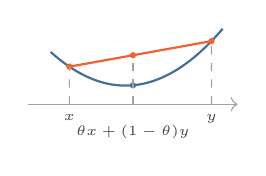
\begin{tikzpicture}[scale=0.95]
  \draw[pgray,->] (-0.2,0) -- (2.6,0);
  \draw[thick,pblue,domain=0.1:2.4,samples=40] plot (\x,{0.45*(\x-1.1)^2+0.25});
  \coordinate (X) at (0.35,{0.45*(0.35-1.1)^2+0.25});
  \coordinate (Y) at (2.25,{0.45*(2.25-1.1)^2+0.25});
  \draw[porange,thick] (X) -- (Y);
  \fill[porange] (X) circle (1.2pt) (Y) circle (1.2pt);
  \draw[dashed,pgray] (0.35,0) node[below,font=\tiny,pdark] {$x$} -- (X);
  \draw[dashed,pgray] (2.25,0) node[below,font=\tiny,pdark] {$y$} -- (Y);
  \fill[pblue] (1.2,{0.45*(1.2-1.1)^2+0.25}) circle (1.2pt);
  \draw[dashed,pgray] (1.2,0) node[below=4pt,font=\tiny,pdark] {$\theta x+(1-\theta)y$} -- (1.2,{(0.45*0.5625+0.25)+(1.2-0.35)/1.9*(0.45*1.3225-0.45*0.5625)});
  \fill[porange] (1.2,{(0.45*0.5625+0.25)+(1.2-0.35)/1.9*(0.45*1.3225-0.45*0.5625)}) circle (1.2pt);
\end{tikzpicture}\\
\note{chord lies above the graph}
\end{minipage}

\topic{Convex function} $f$ (on a convex domain) if for all $\vx,\vy$, $\theta\in[0,1]$:
\[ f(\theta\vx+(1-\theta)\vy)\le\theta f(\vx)+(1-\theta)f(\vy) . \]
1-d is the same with scalars $x,y$. \emph{Strictly} convex: $<$ for $\vx\ne\vy$, $\theta\in(0,1)$.

\topic{Rules for checking convexity}
\begin{itemize}
  \item 1-d: $f''(x)\ge0$ for all $x$ $\iff$ $f$ convex (twice differentiable)
  \item multi-d: $\nabla^2 f(\vx)\succeq0$ (PSD) for all $\vx$ $\iff$ $f$ convex;
        $\nabla^2 f\succ0$ $\Rightarrow$ strictly convex
  \item 1st order: $f(\vy)\ge f(\vx)+\nabla f(\vx)\tr(\vy-\vx)$ (tangent below graph)
  \item preserved by: nonnegative sums $\alpha f+\beta g$, composition with affine map
        $f(\mB\vx+\vy)$, pointwise $\max\{f,g\}$
  \item e.g.\ $\vx\tr\mA\vx$ convex $\iff$ $\mA\succeq0$; \ every norm is convex
\end{itemize}

\sect{Optimality \& Gradient Descent}
\topic{Conditions for a local minimum $\vx^\star$} ($f$ twice differentiable)
\begin{itemize}
  \item \textbf{necessary:} $\nabla f(\vx^\star)=\vzero$ \ and \ $\nabla^2 f(\vx^\star)\succeq0$
  \item \textbf{sufficient:} $\nabla f(\vx^\star)=\vzero$ \ and \ $\nabla^2 f(\vx^\star)\succ0$ (strict local min)
  \item \textbf{convex $f$:} $\nabla f(\vx^\star)=\vzero$ $\iff$ $\vx^\star$ is a \emph{global} minimum
\end{itemize}
1-d: $f'(x^\star)=0$, and $f''(x^\star)\ge0$ (necessary) / $>0$ (sufficient).
\note{Ex.: $\min\tfrac12\vx\tr\mA\vx-\vb\tr\vx$, $\mA\succ0$ $\Rightarrow$ $\vx^\star=\mA\inv\vb$.}

\begin{minipage}[c]{0.6\linewidth}
\topic{Gradient descent} from $\vx_0$ with step size (learning rate) $\alpha>0$:
\[ \vx_{k+1}=\vx_k-\alpha\,\nabla f(\vx_k) \]
Moves against the gradient (steepest descent). Too large $\alpha$ diverges; for
$\tfrac12\vx\tr\mA\vx-\vb\tr\vx$ it converges iff $0<\alpha<2/\lambda_{\max}(\mA)$.
\end{minipage}\hfill
\begin{minipage}[c]{0.38\linewidth}
\centering
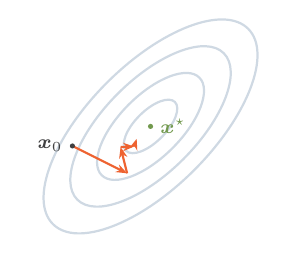
\begin{tikzpicture}[scale=0.62,>={Stealth[length=4pt]}]
  \foreach \c in {0.1,0.4,0.9,1.6}{\draw[plight,thick,rotate=45] (0,0) ellipse ({sqrt(\c/0.2)} and {sqrt(\c)});}
  % GD on f = x'Ax, A = [0.6 -0.4; -0.4 0.6], alpha = 0.7
  \coordinate (p0) at (-1.6,-0.4);
  \coordinate (p1) at (-0.48,-0.96);
  \coordinate (p2) at (-0.614,-0.422);
  \coordinate (p3) at (-0.335,-0.412);
  \coordinate (p4) at (-0.284,-0.253);
  \draw[->,porange,thick] (p0) -- (p1);
  \draw[->,porange,thick] (p1) -- (p2);
  \draw[->,porange,thick] (p2) -- (p3);
  \draw[->,porange,thick] (p3) -- (p4);
  \fill[pdark] (p0) circle (1.5pt) node[left,font=\scriptsize] {$\vx_0$};
  \fill[pgreen] (0,0) circle (1.5pt) node[right,font=\scriptsize] {$\vx^\star$};
\end{tikzpicture}
\end{minipage}

\end{multicols*}
\end{document}

%%% Local Variables:
%%% mode: LaTeX
%%% TeX-master: t
%%% End:
